\chapter{Association Analysis}

Association analysis is a field of techniques aimed at extracting interesting relationships hidden in large datasets. A common application of association analysis is for market basket transactions, which is data referring to purchases done by customers in shops. This data is typically in the form of a set of rows, one per transaction, each containing the set of items bought by a given customer during a single trip. This information can be used to study purchasing habits in order to support a variety of business-related applications, such as marketing promotions, inventory management, and customer relationship management.

\section{Terminology}

Before explaining any algorithm, we need to define some useful terms. As mentioned before, the data is organized into transactions. Let $I$ be the set of all items, and $T$ the set of all transactions. Each transaction $t_i$ contains a number of subsets of $I$, called an \textbf{itemsets}: $t_i = \{ X_1, X_2, \dots, X_n \}$, $X_j = \{ i_1, i_2, \dots, i_k \}$. An itemset containing $k$ items is also called a \textbf{$k$-itemset}. An itemset with no elements is called the null (or empty) itemset. A transaction $t_i$ contains an itemset $X$ if $X$ is a subset of $t_i$.

An important property of an itemset is its support count.

\BoxDef{Support Count}{
The support count of an itemset $X$ is calculated as:
\begin{equation*}
    \sigma(X) = \#\{ t_i | X \subseteq t_i, t_i \in T \}
\end{equation*}
}
In other words, the support count is the number of transactions that contain that itemset. Often, the property of interest is the support.

\BoxDef{Support}{
The support of an itemset $X$ is calculated as:
\begin{equation*}
    s(X) = \dfrac{\sigma(X)}{N}
\end{equation*}
}
An itemset is deemed \textbf{frequent} if its support $s(X)$ is greater than some used-defined minimum threshold, \textit{minsup}.

\BoxDef{Association Rule}{
An association rule is an implication expression between two disjoint itemsets $X$ and $Y$:
\begin{equation*}
    X \rightarrow Y
\end{equation*}
$X$ is called the antecedent, $Y$ the consequent.
}
The strength of an association rule can be measured both in terms of support, and \textbf{confidence}.

\BoxDef{Support of Rule}{
The support of an association rule $X \rightarrow Y$ is calculated as:
\begin{equation*}
    s(X \rightarrow Y) = \dfrac{\sigma(X \cup Y)}{N}
\end{equation*}
}

\BoxDef{Confidence of Rule}{
The confidence of an association rule $X \rightarrow Y$ is calculated as:
\begin{equation*}
    c(X \rightarrow Y) = \dfrac{\sigma(X \cup Y)}{\sigma(X)}
\end{equation*}
}
Support determines how often a rule is applicable to a given dataset, while confidence determines how frequently items in $Y$ appear in transactions that contain $X$.

The goal of association analysis is to extract all rules whose support and confidence are higher than \textit{minsup} and \textit{minconf}, respectively. The brute force approach, in which all possible rules are generated and classified as frequent or infrequent, is highly computationally expensive: for a given dataset of $d$ items, we can list a total of $3^d - 2^{d+1} + 1$ association rules.

Typically, association analysis is broken into two steps: \textbf{frequent itemset generation}, which finds all itemsets with an high enough support, and \textbf{rule generation}, which generates rules based on the frequent itemsets found in the previous step, keeping only the ones with high enough confidence.

\section{Frequent Itemset Generation}

In general, a dataset that contains $k$ items can generate up to $2^k - 1$ itemsets (excluding the empty set). Since $k$ is often very big, the search space of itemsets is too large to be explored exhaustively. The brute-force approach to generate all possible itemsets and calculating support for each of them has a complexity of $O(NMw)$, where $N$ is the number of transactions, $M$ is the number of candidate itemsets, and $w$ is the maximum transaction width (i.e., the number of item a transaction contains). The most common efficient solution to the problem is based on the \textbf{Apriori principle}.

\BoxDef{Apriori principle}{
If an itemset is frequent, then all of its subsets must also be frequent.
}

This principle also implies that if an itemset is infrequent, then all of its supersets will also be infrequent. Consider the example dataset represented by the table below:

\begin{table}[h]
    \centering
    \begin{tabular}{|c|c|}
    \hline
        TID & Items \\
    \hline
        1 & $A$, $B$, $C$ \\
    \hline
        2 & $B$, $D$, $E$, $F$ \\
    \hline
        3 & $C$, $D$, $F$ \\
    \hline
        4 & $B$, $E$, $F$ \\
    \hline
        5 & $A$, $B$, $E$, $F$ \\
    \hline
    \end{tabular}
\end{table}

Assuming a \textit{minsup} threshold of 0.6, the itemset $\{B,E,F\}$ is frequent. The itemsets $\{B,E\}$, $\{B,F\}$, and $\{E,F\}$ are frequent as well. Conversely, $\{A,B\}$ is not frequent, so any itemset obtained by adding items to it will also be infrequent.

The Apriori property holds because of the \textbf{anti-monotone property} of the support measure.

\BoxDef{Anti-monotone property}{
A measure $f$ possesses the anti-monotone property if for every itemset $X$ that is a proper subset of an itemset $Y$, it holds that $f(Y) \leq f(X)$.
}

\subsection{Apriori Algorithm}

The Apriori algorithm uses the Apriori principle to generate all potential frequent itemsets and prune infrequent ones. The pseudocode for the algorithm is presented below.

\begin{algorithm}
\caption{Frequent itemset generation of the Apriori algorithm.}
\begin{algorithmic}[1]
    \State $k = 1$
    \State $F_k = \{ i | i \in I \land s(\{i\}) \geq minsup \}$ \# find all frequent itemsets

    \Repeat
        \State $k = k + 1$
        \State $C_k$ = c\texttt{andidate-gen}($F_{k-1}$) \# generate all candidate itemsets
        \State $C_k$ = \texttt{candidate-prune}($C_k$, $F_{k-1}$) \# prune itemsets with infrequent subsets

        \For{all $t \in T$}
            \State $C_t$ = subsets($C_k$, $t$)

            \For{all $c \in C_t$}
                \State $\sigma(c) = \sigma(c) + 1$ \# increment support count
            \EndFor
        \EndFor
        \State $F_k = \{ c | c \in C_k \land s(c) \geq minsup \}$ \# find all frequent k-itemsets
    \Until{$F_k = \emptyset$}
    \State \Return $\cup F_k$
\end{algorithmic}
\end{algorithm}

The algorithm starts by scanning the dataset and finding all frequent items, constructing the set of frequent 1-itemsets. The main loop can be broken into three different main phases: candidate generation, candidate pruning, and support counting.

\subsubsection{Candidate generation}

This phase generates new candidate $k$-itemsets by ``fusing'' together the frequent $(k-1)$-itemsets found in the previous iteration. The brute-force approach consists in combining all $d$ items to produce all possible $k$-itemsets, but it would result in a total of $\binom{d}{k}$ candidates.

An alternative method for candidate generation is the $F_{k-1} \times F_1$ method. Each frequent $(k-1)$-itemset is extended with frequent items that are not part of the $(k-1)$-itemset. This procedure is complete, since every frequent $k$-itemset is composed of a frequent $(k-1)$-itemset and a frequent 1-itemset. All frequent $k$-itemsets are contained within the candidate $k$-itemsets generated. Still, this procedure produces a large number of unnecessary candidates, and can produce duplicate candidates as well.

Another method is the $F_{k-1} \times F_{k-1}$ method, which is the one actually used by the Apriori algorithm. The set of candidate $k$-itemsets is obtained by merging together pairs of frequent $(k-1)$-itemsets. A pair is merged only if their first $k-2$ items, sorted lexicographically, perfectly match. More formally: let $A = \{ a_1, a_2, \dots, a_{k-1} \}$ and $B = \{ b_1, b_2, \dots, b_{k-1} \}$ be two frequent $(k-1)$-itemsets. $A$ and $B$ can be merged if and only if:
\begin{equation*}
    a_i = b_i \,, i \in [1,k-2] \,.
\end{equation*}
This method is both complete and guaranteed to never generate duplicates.

\subsubsection{Candidate pruning}

Pruning removes all the candidate $k$-itemsets that contain at least one infrequent subset (since as per the Apriori principle, those $k$-itemsets will certainly be infrequent as well). So, for a given candidate $k$-itemset $X = \{ i_1, i_2, \dots, i_k \}$, the procedure checks if any itemset $X - \{i_j\}$ does not appear in the set of frequent $(k-1)$-itemsets. For the specific case of the $F_{k-1} \times F_{k-1}$ method, the pruning procedure only needs to check $k-2$ subsets for each candidate, since two of its $(k-1)$ subsets (the ones merged to generate it) are already known to be frequent.

\subsubsection{Support counting} 

Support counting simply iterates over all the transactions in the dataset and increases the support count of the candidate itemsets contained into each of them. The brute-force approach to counting is to compare each transaction against every single candidate itemset, but, as always, this is computationally expensive.

The method followed by Apriori exploits a prefix tree structure to find the candidates contained in a transaction. The root of the tree corresponds to the full transaction $t = \{ i_1, 1_2, \dots, \i_n \}$. Assuming that each itemset keeps its items always in increasing lexicographic order, an itemset can be enumerated by specifying the smallest item first, followed by the larger ones. So, given a transaction $t = \{ 1, 2, 3, 4, 5 \}$, all 3-itemsets can only start with either 1, 2, or 3. The root will have three children at level 1, one for each ``starting'' item. The same thing can be repeated to produce level 2. If 1 is the first item of the 3-itemset, it can be only followed by 2, 3, or 4, but not 5, since then it could not have a total of 3 items. The node that ``starts'' with 1 will have three children, the one that ``starts'' with 2 will have two children, and finally the node ``starting'' with 3 will only have one child. This process is repeated until all leaf nodes containing all possible $k$-itemsets contained in the transaction are reached. The support of all the itemsets found is simply increased by 1.

Below is the prefix tree generated with the above example.

\begin{figure}[h]
    \centering
    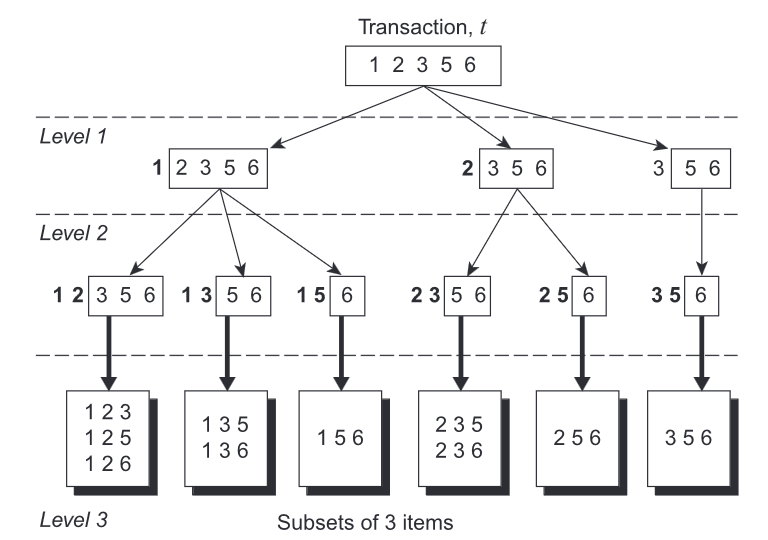
\includegraphics[width=0.7\linewidth]{img/apriori_prefixtree.png}   
\end{figure}

\section{Rule Generation}

Each frequent $k$-itemset, $Y$, can produce up to $2^k - 2$ association rules, excluding rules with empty antecedents or consequents. An association rule can be extracted by partitioning the itemset $Y$ into two non empty subsets, $X$ and $Y-X$, such that $c(X \rightarrow Y-X)$ is greater than \textit{minconf}. Computing the confidence of an association rule does not require additional scans of the transaction dataset. The itemsets from which rules are extracted from are all frequent, and so are their subsets. Below is the pseudocode of the algorithm.

\begin{algorithm}[h]
\caption{Rule generation of the Apriori algorithm.}
\begin{algorithmic}[1]
    \State $k = 2$
    \For{each frequent $k$-itemset $f_k$}
        \State $H_1 = \{ i | i \in f_k \}$
        \State \texttt{ap-genrules}($f_k, H_1$)
    \EndFor
\end{algorithmic}
\end{algorithm}

\begin{algorithm}[h]
\caption{Procedure \texttt{ap-genrules}($f_k, H_m$).}
\begin{algorithmic}[1]
    \State $k = |f_k|$
    \State $m = |H_m|$

    \If{$k > m+1$}
        \State $H_{m+1}$ = \texttt{candidate-gen}($H_m$)
        \State $H_{m+1}$ = \texttt{candidate-prune}($H_{m+1}, H_m$)

        \For{each $h_{m+1} \in H_{m+1}$}
            \State $conf = \sigma(f_k) / \sigma(f_k - h_{m+1})$
            \If{$conf \geq minconf$}
                \State \Return $(f_k - h_{m+1}) \rightarrow h_{m+1}$
            \Else
                Delete $h_{m+1}$ from $H_{m+1}$
            \EndIf
        \EndFor
        \texttt{ap-genrules}($f_k, H_{m+1}$)
    \EndIf
\end{algorithmic}
\end{algorithm}

The process followed by the algorithm to generate new rules is similar to the one seen previously. Initially, only the rules with one item in the consequent are extracted from the frequent itemsets, and the rules with a too low confidence are discarded. The remaining rules are merged to generate new candidate rules: each pair of rules generates a new one by merging the consequents of both. The rules with low confidence are again discarded, and the procedure continues until it generates all rules of high confidence (up to those with only one item in the antecedent).

\section{Compact Representation of Frequent Itemsets}

The number of frequent itemsets generated from a transaction dataset can be very large, so it's useful to identify a small representative set of frequent itemsets from which all other frequent itemsets can be derived. Two such representations are presented in this section.

\subsection{Maximal Frequent Itemsets}

\BoxDef{Maximal frequent itemset}{
A frequent itemset is maximal if none of its immediate supersets is frequent.
}

If we only store maximal frequent itemsets, all other frequent itemsets can be easily extracted since they will be their subsets. This representation is especially useful for datasets that produce very long frequent itemsets, as there are exponentially more frequent itemsets in such data. However, maximal frequent itemsets do not contain the support information of their subsets, so an additional pass over the data is needed to determine the support counts of non-maximal frequent itemsets.

\subsection{Closed Itemsets}

\BoxDef{Closed itemset}{
An itemset $X$ is closed if none of its immediate supersets has exactly the same support count as $X$.
}

\BoxDef{Closed frequent itemset}{
An itemset is a closed frequent itemset if it is closed and its support is greater than or equal than \textit{minsup}.
}

Closed frequent itemsets provide a minimal representation while still keeping support information about all frequent itemsets. If we know their support counts, we can derive the support count of any other itemset. Starting from the longest frequent itemsets, for each set of frequent $k$-itemsets, and for each non-closed itemset $f$ in that set, the support count is calculated as:
\begin{equation*}
    f.sup = \max\{f'.sup : f' \in F_{k+1}, f \subset f'\}
\end{equation*}

\section{Pattern Evaluation}

Association analysis algorithms can still generate huge amounts of frequent rules. Not all of those rules may be interesting, however. There is a need to establish some set of \textbf{objective interestingness measures}, that can be used to rank patterns in terms of how much or how little they are interesting. Afterwards, we need to establish some \textbf{subjective measures}, that measure how actually useful a pattern can be in revealing unexpected relationships among data.

\subsection{Objective Measures of Interestingness}

An objective measure is a data-driven approach for evaluating the quality of association patterns. It is domain independent, and the user only needs to set a minimum threshold to filter out low-quality patterns. An objective measure is usually calculated using the frequency counts reported into a \textbf{contingency table}.

\begin{table}[h]
    \centering
    \begin{tabular}{c|ccc}
         & $B$ & $\Bar{B}$ & \\
        \hline
        $A$ & $f_{11}$ & $f_{10}$ & $f_{1+}$\\
        $\Bar{A}$ & $f_{01} $ & $f_{00}$ & $f_{0+}$\\
        & $f_{+1}$ & $f_{+0}$ & $N$ \\
    \end{tabular}
    \caption{Contingency table for variables $A$ and $B$.}
\end{table}

Each entry $f_{ij}$ in the table indicates a frequency count; e.g., $f_{11}$ indicates the amount of times both $A$ and $B$ appear inside a transaction, while $f_{10}$ indicates the number of times $A$ appears but not $B$.

Support and confidence are two measures that can be derived from such table. However, they are not infallible; support may still exclude some interesting patterns in the data that involve low support items, and confidence does not necessarily guarantee that a rule is reasonable. To better illustrate this last issue, look at the example in the table below.

\begin{table}[h]
    \centering
    \begin{tabular}{c|ccc}
         & $Coffee$ & $\Bar{Coffee}$ & \\
         \hline
         $Tea$ & 150 & 50 & 200 \\
         $\Bar{Tea}$ & 650 & 150 & 800 \\
         & 800 & 200 & 1000 \\
    \end{tabular}
\end{table}

Assume we want to evaluate the association $\{Tea\} \rightarrow \{Coffee\}$: people who drink tea also drink coffee. The rule's support is 15\% (150/1000), and its confidence is 75\% (150/200). However, the total fraction of people who drink coffee is 80\%, while the fraction of tea drinkers who drink coffee is only 75\%. This means that knowing that a person drinks tea actually lowers the probability of that same person being a coffee drinker.

The limitations of confidence can be better expressed in a statistical way. The support of a variable measures the probability of its occurrence, while the support of $\{A,B\}$ measures the probability of the two items occurring together. So, the joint probability can be expressed as follows:
\begin{equation*}
    P(A,B) = s(A,B) = \dfrac{f_{11}}{N}\,.
\end{equation*}
If $A$ and $B$ are statistically independent, then $P(A,B) = P(A) \times P(B)$, so we can rewrite the above equation as:
\begin{equation*}
    P(A,B) = s(A,B) = \dfrac{f_{1+}}{N} \times \dfrac{f_{+1}}{N}\,.
\end{equation*}
If the supports between two variables calculated in the two ways shown above are the same, then the variables are independent, while if they are very different it means the two variables are dependent. Since the confidence measure considers the deviance of $s(A,B)$ from $s(A)$, but not from $s(A) \times s(B)$, it does not really detect spurious patterns, and potentially rejects interesting ones.

Some other objective measures that take this into account are defined below.
\BoxDef{Lift}{
\begin{equation*}
    Lift(X,Y) = \dfrac{P(Y|X)}{P(Y)} = \dfrac{s(X \rightarrow Y)}{s(Y)}
\end{equation*}
}

\BoxDef{Interest}{
\begin{equation*}
    I(X,Y) = \dfrac{P(X,Y)}{P(X)P(Y)} = \dfrac{f_{11}}{s(X) \times s(Y)}
\end{equation*}
}
Lift and interest are essentially the same measure, but lift is used for association rules, while interest is used for itemsets.

\BoxDef{Piatesky-Shapiro}{
\begin{equation*}
    PS(X,Y) = P(X,Y) - P(X)P(Y) = s(f_{11}) - s(X) \times s(Y)
\end{equation*}
}

\BoxDef{$\phi$-coefficient}{
\begin{gather*}
    \phi(X,Y) = \dfrac{P(X,Y) - P(X)P(Y)}{\sqrt{P(X)(1-P(X)) P(Y)(1-P(Y))}} = \\
    = \dfrac{f_{11} - s(X) \times s(Y)}{\sqrt{s(X)(1-s(X)) \times s(Y)(1-P(Y))}}
\end{gather*}
}

\section{Multi-Level Association Rules}

A \textbf{concept hierarchy} is a multilevel organization of the entities defined withing a particular domain. For example, a concept hierarchy can be an item taxonomy describing relationships between items in market basket data: milk and bread are a type of food, DVD is a type of home electronics item. Concept hierarchies can be defined on the basis of some domain-specific knowledge or based on a standard classification scheme defined by certain organizations.

A concept hierarchy can be defined using a directed acyclic graph; if there is an edge going from a node $p$ to a node $c$, then $p$ is the parent of $c$, and $c$ is the child of $p$. If there is a path that goes from node $a$ to node $d$, then $a$ is the ancestor of $d$, and $d$ is the descendant of $a$.

The main advantages of incorporating concept hierarchies into association analysis are related to the fact that items at lower levels of the hierarchy may not have enough support to appear as frequent, but if they are incorporated into higher level concepts, they can contribute to the analysis. On the flip side, rules obtained from itemsets with items from higher levels of the hierarchy may be too generic, and/or have too low confidence, so being able to use more specific concepts may highlight interesting relationships. Rules found at the lower levels of the hierarchy tend to be too specific and may not be as interesting as rules found at higher levels.

To handle concept hierarchies, we can consider two approaches:
\begin{itemize}
    \item Extending the current association rule formation by adding higher level items to each transaction; i.e., $\{ whole\_milk, wheat\_bread \}$ becomes $\{ whole\_milk, wheat\_bread, milk, bread, food \}$. However, items at higher levels will have much higher support counts, and if the chosen $minsup$ threshold is too low, there will be too many frequent itemsets involving high-level items. Additionally, this approach increases the dimensionality of the data, making transactions actually longer.

    \item Generating frequent patterns at highest levels first; then, generating frequent patterns at the next highest level lower than the previous one, and so on. While this method will surely find all patterns for all hierarchy levels, it's very costly as it passes multiple times over the data (once for each level), and does not capture cross-level association patters. 
\end{itemize}

\section{FP-Growth}

Apriori is an historically significant algorithm for pattern mining, but it suffers from a series of inefficiencies. The biggest bottleneck is represented by candidate generation. Especially during the first iterations, the number of candidates increases exponentially, and each of those candidates will have to be evaluated for pruning and eventually have its support calculated. Specifically, if $n$ is the length of the longest pattern, the algorithm will need $n+1$ scans of the dataset.

FP-Growth (``Frequent Pattern Growth'') is a more efficient algorithm that follows a different approach to extract frequent itemsets. The dataset is encoded using a compact data structure called \textbf{FP-Tree}, and extracts frequent itemsets directly from this structure instead of generating them in a bottom-up way like Apriori does.

\subsection{FP-Tree Representation}

The first step of the algorithm consist in constructing the FP-tree that represents the input data.
\begin{enumerate}
    \item The dataset is scanned to calculate the support count of each item, and infrequent items are discarded. All frequent ones are sorted on the basis of their support count in descending order within each transaction of the dataset.

    \item Each transaction is read and nodes are gradually added to the tree, mapping each transaction. The tree always starts with an empty root ($\{\}$). The first transaction is read, and items are added as nodes so that the first item found is the child of the root, the second is the child of the first item, and so on, setting their support count to 1. As the second transaction is read, new nodes are added or existing nodes' support counts are increased. Additionally, if multiple paths share the same items, the corresponding nodes are linked one to the other.
\end{enumerate}

This data structure is both \textbf{complete} (it correctly maps all transactions in the dataset, preserving all information needed for pattern mining), and \textbf{compact} (it reduces irrelevant information and is never larger than the original dataset).

\subsection{Mining Frequent Itemsets From FP-Trees}

Once the tree has been constructed, the algorithm can extract all the frequent itemsets in the database, employing a divide-and-conquer strategy. The mining starts from single items and gradually builds longer itemsets.
\begin{enumerate}
    \item All the prefix paths containing a certain item $i$ are gathered.

    \item The support count of that item is obtained by adding the support counts associated with the nodes that are related to that item. If its support is higher than $minsup$, the item is declared a frequent 1-itemset, and the algorithm proceeds to the next step, trying to find frequent itemsets ending in $i$.

    \item All the subproblems involving $i$ and one other item are solved; e.g., if the node-link paths in the FP-tree that end in $i$ involve the items $j$, $k$, and $l$, the algorithm will try to find frequent itemsets ending in $ji$, $ki$, and $li$. Before solving these subproblems, the prefix paths found in the first step are converted into a \textbf{conditional FP-tree}. This tree is obtained in the following way:
        \begin{enumerate}
            \item All paths are truncated,  excluding the item $i$, since we already know all these paths are relative to that specific item.
            
            \item The support counts along the paths are updated since they may include counts that involve transactions without $i$. This step constructs the \textbf{conditional pattern base} of item $i$.

            \item Some of the items may now be infrequent, and are therefore removed from the structure.
        \end{enumerate}

    \item To find all frequent itemsets ending in $ji$, the prefix paths for $j$ are gathered from the conditional FP-tree that was just constructed. By adding the frequency counts associated with $j$, we obtain the support count of $ji$. The algorithm then constructs the conditional FP-tree for $ji$ using the same procedure as before; it gathers all prefix paths ending in $j$, truncates the last node, and updates the support counts of each item, removing infrequent ones if needed. After itemsets ending in $ji$ are identified, the algorithm can continue by generating conditional FP-trees for three-item itemsets, or alternatively continue to a different two-item itemset if no more prefix paths are found.
\end{enumerate}

FP-growth is an order of magnitude faster than Apriori. It does not generate and test candidates and uses a compact data structure that does not require multiple passes over the dataset.